\chapter{Ziel- und Anforderungsanalyse}
\label{CHAP:REQUIREMENTS}

Nachdem die Grundlagen für die weiteren Ausführungen geschaffen wurden, wird nachfolgend der thematische Umfang der Arbeit eingegrenzt. Anschließend werden die Ziele und Anforderungen der betrachteten Anwendungsdomäne ausgeführt.

\section{Thematische Eingrenzung}

Derzeitige Web3D-Technologien können anhand ihrer grundsätzlichen technischen Ausprägung grob in zwei Kategorien eingeteilt werden \autocite{Jankowski:2013:DII:2466533.2466547}. Vertreter des deklarativen Paradigmas bauen auf bestehende Webstandards auf und realisieren eine 3D-Darstellung mittels eines hierarchischen, direkt in HTML eingebundenen Szenengraphen. Kindelemente des Szenengraphen stellen hierbei die Objekte der 3D-Szene dar und werden in XML-ähnlicher Notation direkt innerhalb des \emph{Document Object Models} integriert. Diesem Ansatz gegenüber stehen imperative Ansätze, welche auf einem deutlich niedrigeren Abstraktionsniveau angesiedelt sind und generell eine größere Hardwärenähe aufweisen. Ähnlich zu klassischen Grafikbibliotheken wie \emph{OpenGL} und \emph{Direct3D} wird die eigentliche Grafikprogrammierung hier durch explizite Einzelschritte auf Vertex- und Polygonebene umgesetzt.

Mit dem durch das Web3D Consortium entwickelten ISO-""Standard \emph{Extensible 3D} (X3D) und dem zugehörigen Framework \emph{X3DOM} wird zunächst ein Repräsentant des deklarativen Modells betrachtet. Bei X3D handelt sich um eine XML-basierte Beschreibungssprache für die Darstellung webbasierter 3D-""Grafik. X3DOM stellt ein JavaScript-basiertes Integrationsmodell für X3D in HTML dar.

Im Anschluss wird die \emph{Web Graphics Library} (WebGL) als Vertreter einer imperativen Grafikbibliothek erörtert. WebGL basiert auf der \emph{Open Graphics Library for Embedded Systems 2.0} (OpenGL ES), ein auf Mobilgeräte abgestimmter Dialekt von \emph{OpenGL 2.0} \autocite{KHRONOS_OPENGL_ES_20_SPEC}. Die Bibliothek wurde hierbei von zahlreichen Altlasten wie Funktionen der Fixed-Rendering-Pipeline befreit. OpenGL ist eine weit verbreitende plattformunabhängige Spezifikation für 2D- und 3D-Computergrafikanwendungen \autocite{OPENGL_ABOUT}. Die Schnittstelle zwischen WebGL und dem Webbrowser wird dabei durch JavaScript realisiert.

Eine weiterer derzeitige Ansatz für 3D-""Darstellung im Webbrowser ist die von Adobe als Bestandteil ihrer proprietären Multimedia-Plattform \emph{Flash} entwickelte Technologie \emph{Stage 3D}. Obgleich Flash im Desktop-Bereich äußerst verbreitet ist, ist eine Unterstützung auf den vorherrschenden mobilen Betriebssystemen \emph{Android} und \emph{iOS} gar nicht oder nur nach Installation entsprechender Software möglich \autocite{Evans201443}. Aufgrund dieses Umstands und des Fokus der Arbeit auf offene Standards ist Stage 3D daher nicht Bestandteil der Untersuchung.

\section{Charakterisierung der Anwendungsdomäne}
\label{SEC:APPLICATION_DOMAIN}

Bevor die angestrebten Ziele und Testkriterien der Evaluation formuliert werden können, muss zunächst die grundsätzliche Natur der untersuchten Klasse von 3D-""Anwendung charakterisiert werden, um eine Vorstellung für deren spezifische Anforderungen zu schaffen. Mittels exemplarischer Anwendungsfälle wird die Anwendungsdomäne konkretisiert und erleichtert die nachfolgende Analyse:

\begin{enumerate}[noitemsep]
	\item Darstellung von Produkten in Web-Shops und auf Hersteller-""Websites mittels eingebetteter 3D-""Modelle: Interessierte Kunden können die Ansicht interaktiv durch Klicken und Ziehen anpassen und das Produkt so von allen Seiten detailgenau betrachten. Falls es verschiedene Ausführungen des Artikels wie Farbe oder Material gibt, so kann dies dynamisch verändert werden.
	\item Virtuelle Repräsentation von Ausstellungsstücken im Kulturbereich: Einige Museen und andere kulturelle Einrichtungen nutzen heutzutage 3D-""Scanner zur Katalogisierung ihrer Exponate. Diese 3D-""Modelle können auf Websites eingebunden werden und anderen auf diesem Gebiet forschenden Experten so zur Verfügung gestellt werden.
	\item Visualisierung wissenschaftlicher Modelle im akademischen und schulischen Umfeld wie beispielsweise die Darstellung von Anatomie in der Medizin oder die Abbildung komplexer Moleküle in der Chemie: Studenten und Schüler können durch Erforschen der 3D-""Darstellung die Zusammenhänge und räumlichen Verhältnisse des gezeigten Sachverhalts selbstständig erfassen. Darüber hinaus können Konzepte mittels Animationen und der Möglichkeit, einzelne Darstellungsebenen auszublenden, sehr gut veranschaulicht werden.
\end{enumerate}

Explizit nicht Teil der weiteren Betrachtung sind browserbasierte Computerspiele, da diese für sich ein sehr weitläufiges Thema darstellen und den Umfang der Arbeit überschreiten.

\section{Technische Anforderungen}

\subsection{Browserunterstützung und Plattformunabhängigkeit}
Um eine webbasierte 3D-""Anwendung einer möglichst großen Zielgruppe zugänglich zu machen, ist die grundsätzliche Unterstützung der 3D-""Technologie innerhalb des Webbrowsers und des Betriebssystems notwendig. Abbildung \ref{FIG_BROWSER_MARKETSHARE} zeigt die Entwicklung der weltweiten Marktanteile\footnote{Aufgrund der Schnelllebigkeit des World Wide Webs sind Aussagen über die tatsächlichen Marktanteile von Webbrowsern grundsätzlich schwierig zu treffen und stets mit Unschärfe versehen.} von Webbrowsern auf Desktop- und Mobilgeräten innerhalb des Zeitraums von Januar 2009 bis April 2014.

\begin{figure}[ht]
	\centering
	\footnotesize
	% GNUPLOT: LaTeX picture with Postscript
\begingroup
  \makeatletter
  \providecommand\color[2][]{%
    \GenericError{(gnuplot) \space\space\space\@spaces}{%
      Package color not loaded in conjunction with
      terminal option `colourtext'%
    }{See the gnuplot documentation for explanation.%
    }{Either use 'blacktext' in gnuplot or load the package
      color.sty in LaTeX.}%
    \renewcommand\color[2][]{}%
  }%
  \providecommand\includegraphics[2][]{%
    \GenericError{(gnuplot) \space\space\space\@spaces}{%
      Package graphicx or graphics not loaded%
    }{See the gnuplot documentation for explanation.%
    }{The gnuplot epslatex terminal needs graphicx.sty or graphics.sty.}%
    \renewcommand\includegraphics[2][]{}%
  }%
  \providecommand\rotatebox[2]{#2}%
  \@ifundefined{ifGPcolor}{%
    \newif\ifGPcolor
    \GPcolortrue
  }{}%
  \@ifundefined{ifGPblacktext}{%
    \newif\ifGPblacktext
    \GPblacktexttrue
  }{}%
  % define a \g@addto@macro without @ in the name:
  \let\gplgaddtomacro\g@addto@macro
  % define empty templates for all commands taking text:
  \gdef\gplbacktext{}%
  \gdef\gplfronttext{}%
  \makeatother
  \ifGPblacktext
    % no textcolor at all
    \def\colorrgb#1{}%
    \def\colorgray#1{}%
  \else
    % gray or color?
    \ifGPcolor
      \def\colorrgb#1{\color[rgb]{#1}}%
      \def\colorgray#1{\color[gray]{#1}}%
      \expandafter\def\csname LTw\endcsname{\color{white}}%
      \expandafter\def\csname LTb\endcsname{\color{black}}%
      \expandafter\def\csname LTa\endcsname{\color{black}}%
      \expandafter\def\csname LT0\endcsname{\color[rgb]{1,0,0}}%
      \expandafter\def\csname LT1\endcsname{\color[rgb]{0,1,0}}%
      \expandafter\def\csname LT2\endcsname{\color[rgb]{0,0,1}}%
      \expandafter\def\csname LT3\endcsname{\color[rgb]{1,0,1}}%
      \expandafter\def\csname LT4\endcsname{\color[rgb]{0,1,1}}%
      \expandafter\def\csname LT5\endcsname{\color[rgb]{1,1,0}}%
      \expandafter\def\csname LT6\endcsname{\color[rgb]{0,0,0}}%
      \expandafter\def\csname LT7\endcsname{\color[rgb]{1,0.3,0}}%
      \expandafter\def\csname LT8\endcsname{\color[rgb]{0.5,0.5,0.5}}%
    \else
      % gray
      \def\colorrgb#1{\color{black}}%
      \def\colorgray#1{\color[gray]{#1}}%
      \expandafter\def\csname LTw\endcsname{\color{white}}%
      \expandafter\def\csname LTb\endcsname{\color{black}}%
      \expandafter\def\csname LTa\endcsname{\color{black}}%
      \expandafter\def\csname LT0\endcsname{\color{black}}%
      \expandafter\def\csname LT1\endcsname{\color{black}}%
      \expandafter\def\csname LT2\endcsname{\color{black}}%
      \expandafter\def\csname LT3\endcsname{\color{black}}%
      \expandafter\def\csname LT4\endcsname{\color{black}}%
      \expandafter\def\csname LT5\endcsname{\color{black}}%
      \expandafter\def\csname LT6\endcsname{\color{black}}%
      \expandafter\def\csname LT7\endcsname{\color{black}}%
      \expandafter\def\csname LT8\endcsname{\color{black}}%
    \fi
  \fi
  \setlength{\unitlength}{0.0500bp}%
  \begin{picture}(7200.00,4320.00)%
    \gplgaddtomacro\gplbacktext{%
      \csname LTb\endcsname%
      \put(595,636){\makebox(0,0)[r]{\strut{} 0}}%
      \csname LTb\endcsname%
      \put(595,1137){\makebox(0,0)[r]{\strut{} 10}}%
      \csname LTb\endcsname%
      \put(595,1638){\makebox(0,0)[r]{\strut{} 20}}%
      \csname LTb\endcsname%
      \put(595,2139){\makebox(0,0)[r]{\strut{} 30}}%
      \csname LTb\endcsname%
      \put(595,2640){\makebox(0,0)[r]{\strut{} 40}}%
      \csname LTb\endcsname%
      \put(595,3141){\makebox(0,0)[r]{\strut{} 50}}%
      \csname LTb\endcsname%
      \put(595,3642){\makebox(0,0)[r]{\strut{} 60}}%
      \csname LTb\endcsname%
      \put(595,4143){\makebox(0,0)[r]{\strut{} 70}}%
      \csname LTb\endcsname%
      \put(683,437){\makebox(0,0){\strut{}2009}}%
      \csname LTb\endcsname%
      \put(1875,437){\makebox(0,0){\strut{}2010}}%
      \csname LTb\endcsname%
      \put(3067,437){\makebox(0,0){\strut{}2011}}%
      \csname LTb\endcsname%
      \put(4258,437){\makebox(0,0){\strut{}2012}}%
      \csname LTb\endcsname%
      \put(5450,437){\makebox(0,0){\strut{}2013}}%
      \csname LTb\endcsname%
      \put(6642,437){\makebox(0,0){\strut{}2014}}%
      \csname LTb\endcsname%
      \put(143,2389){\rotatebox{-270}{\makebox(0,0){\strut{}Prozent}}}%
      \csname LTb\endcsname%
      \put(3809,139){\makebox(0,0){\strut{}Jahr}}%
    }%
    \gplgaddtomacro\gplfronttext{%
      \csname LTb\endcsname%
      \put(6240,3965){\scriptsize\sffamily\makebox(0,0)[r]{\strut{}Internet Explorer}}%
      \csname LTb\endcsname%
      \put(6240,3766){\scriptsize\sffamily\makebox(0,0)[r]{\strut{}Chrome}}%
      \csname LTb\endcsname%
      \put(6240,3567){\scriptsize\sffamily\makebox(0,0)[r]{\strut{}Firefox}}%
      \csname LTb\endcsname%
      \put(6240,3368){\scriptsize\sffamily\makebox(0,0)[r]{\strut{}Safari}}%
      \csname LTb\endcsname%
      \put(6240,3169){\scriptsize\sffamily\makebox(0,0)[r]{\strut{}Opera}}%
      \csname LTb\endcsname%
      \put(6240,2970){\scriptsize\sffamily\makebox(0,0)[r]{\strut{}Mobile Browser}}%
    }%
    \gplbacktext
    \put(0,0){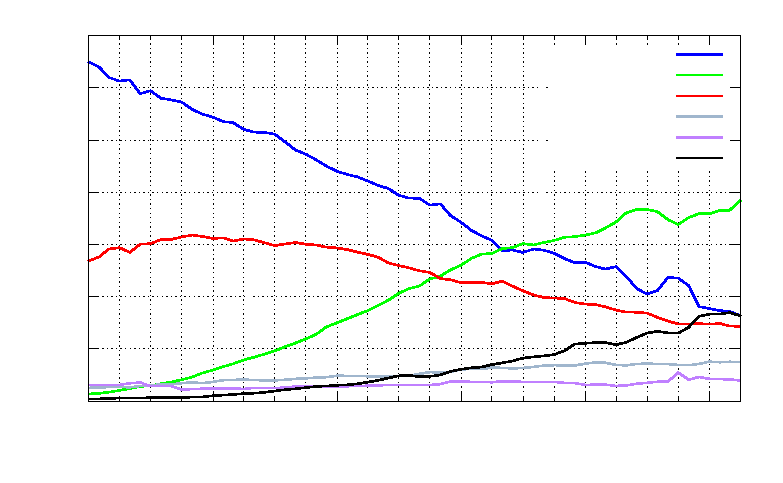
\includegraphics{kap3/figures/browser-ww-monthly-200901-201404-with-mobile}}%
    \gplfronttext
  \end{picture}%
\endgroup

	\caption{Marktanteil von Webbrowsern weltweit \autocite{STATCOUNTER_BROWSERS_09_14}.}
	\label{FIG_BROWSER_MARKETSHARE}
\end{figure}

Deutlich erkennbar ist ein kontinuierlich starker Rückgang des Microsoft Internet Explorers von ehemals 65,0\% zu Anfang des Jahres 2009 auf nur noch 16,4\% im April 2014. Gleichzeitig stieg der Marktanteil von Google Chrome seit dessen Erscheinungsjahr 2008 stetig auf 38,3\% an. Seit 2011 ist Firefoxs Anteil rückläufig und reduzierte sich annähernd um die Hälfte von 26,7\% auf 14,3\%. Während sich Safari auf niedrigem Niveau von 2,6\% auf 7,5\% leicht steigern konnte, weist Operas Kurve nur geringfügige Veränderungen auf. Innerhalb des betrachteten Zeitraums stieg der Anteil hier von 3,1\% auf 4,0\%.
Das Diagramm zeigt zudem eine signifikante Zunahme von mobilen Webbrowsern, die einen klaren Trend hin zur mobilen Nutzung des Webs belegen. So stieg dieser Anteil von 0,4\% stetig auf 16,4\%, was fast einem Sechstel aller Zugriffe entspricht. Eine Erhebung des Statistischen Bundesamts aus dem Jahr 2013 stützt diese These: 2013 nutzten 51\% aller Internetbenutzer im Alter ab 10 Jahren in Deutschland das mobile Internet \autocite{DESTATIS_MOBILE_INTERNET_USERS}.

% anhand - aufgrund
Auf Basis dieser Daten definiert sich die erste Zielvorgabe: Die nähere Überprüfung der Unterstützung der betrachteten 3D-""Technologie innerhalb der fünf meistverwendesten Desktop-Browsern, also Chrome, Internet Explorer, Firefox, Safari und Opera. Je nach Verfügbarkeit der Browser werden diese auf den drei verbreitesten Betriebssystemen, Microsoft Windows, Apple Mac OS X und GNU/Linux getestet.

Aufgrund des wie in Abbildung \ref{FIG_BROWSER_MARKETSHARE} gezeigten, zunehmend stärkeren Einflusses mobiler Geräte stellt deren Untersuchung hinsichtlich dieses Kriteriums ebenso eine Anforderung dar. Betrachtet werden hierbei das hauptsächlich durch Google entwickelte freie Betriebssystem \emph{Android} und Apples mobile Plattform \emph{iOS}.

\subsection{Vermeidung von Browser-Plugins}
Eine weitere Anforderung stellt die Darstellung der 3D-""Szene unter Vermeidung zusätzlicher Browser-Plugins von Drittherstellern dar. In der langjährigen Geschichte von Web3D gab es zahlreiche Plugin-basierte Ansätze, die sich allesamt langfristig nicht behaupten konnten \autocite{Evans201443}.

Sofern eine explizite Aktion seitens des Benutzers, etwa das Installieren eines Browser-Plugins nötig ist, um eine Webseite mit eingebetter 3D-""Grafik zu betrachten, stellt dies eine Einstiegshürde für den Webauftritt dar und kann dessen Benutzerakzeptanz senken. Viele Benutzer stehen Plugins generell eher skeptisch gegenüber, da sie unbekannte Software darstellen, was häufig von Laien als eine potentielle Gefährdung ihres Computers erachtet wird. Zudem sind Plugins oftmals mühsam zu verwalten sind \autocite{Ortiz:2010}.
Das Installieren von Software verlangt zudem eine gewisse Fachkompetenz des Benutzers, die nicht immer gegeben ist. Dies ist in Anwendungsdomänen wie Schulen, Universitäten und Firmen darüber hinaus aufgrund mangelnder Administrationsrechte grundsätzlich nicht möglich.

Veraltete oder wenig verbreitete Browser-Plugins können tatsächlich ein nicht unerhebliches Sicherheitsrisiko innerhalb des Browsers darstellen, da unentdeckte Schwachstellen innerhalb des Plugin-Codes von Angreifern ausgenutzt werden können (\emph{Exploits}) \autocite{Ortiz:2010}. Weiterhin können Browser-Plugins zu Abstürzen der Software führen. Sowohl Google Chrome als auch Mozilla Firefox führen aufgrund dieser möglichen Sicherheits- und Stabilitätsprobleme zahlreiche als unsicher erachtete Plugins erst nach expliziter Autorisierung des Benutzers aus \autocite{CHROME_BLOCKED_PLUGINS} \autocite{FIREFOX_BLOCKED_PLUGINS}.

Aufgrund all dieser Unzulänglichkeiten von Browser-Plugins sind diese als Abhängigkeit einer Web3D-""Anwendung zu vermeiden.

\subsection{Vergleich der Hard"-ware-Anforderungen}
\label{SECTION:HARDWARE_REQUIREMENTS}

Ebenso entscheidend für die Alltagstauglichkeit und Benutzerakzeptanz der 3D-""Applikation ist deren Hard"-ware-""Anforderung und die generelle \emph{Performance} bei der Darstellung. Da letztere in erster Linie von der verfügbaren Grafik-Hardware abhängt, ist eine absolute Bewertung der Leistungsfähigkeit von X3DOM und WebGL schwierig vorzunehmen. Für die Bewertung der zwei Technologien müssen diese einander daher auf demselben Testsystem gegenüber gestellt werden, um vergleichbare Aussagen bezüglich ihrer Performance treffen zu können. In der Evaluation soll diese auf verschiedenen Betriebssystemen und Webbrowsern verglichen werden.

\begin{figure}[!h]
	\centering
	\includegraphics[width=0.5\textwidth]{kap3/figures/hw-top-ten-resolutions-steam-crop.pdf}
	\caption{Zehn meistgenutzte Bildschirmauflösungen auf Steam \autocite{STEAM_HARDWARE_SURVERY}.}
	\label{STEAM_HW_RESOLUTIONS}
\end{figure}

Weiterhin besitzt die Bildschirmauflösung großen Einfluss auf die Hard"-ware-""Anforderung der 3D-""Anwendung, da sich der Berechnungsaufwand während des Renderings durch die höhere Pixelanzahl vergrößert. Abbildung \ref{STEAM_HW_RESOLUTIONS} zeigt die zehn häufigsten Bildschirmauflösungen innerhalb der Spieleplattform Steam des amerikanischen Spieleentwicklers Valve Cooperation im April 2014. Die Statistik entstammt einer nicht repräsentativen monatlich durchgeführten Hard"-ware-Umfrage innerhalb dieses Netzwerks. Die mit Abstand am häufigsten gemessenen Bildschirmauflösungen sind 1920 x 1080 Pixel (\emph{FullHD}) und 1366 x 768 Pixel. Als weiteres Kriterium der Evaluation wird daher die Untersuchung des Einflusses der nachfolgend aufgelisteten fünf Bildschirm-Auflösungen auf die Performance spezifiziert.

\begin{itemize}[noitemsep]
	\item 1024 x 768
    \item 1280 x 1024
	\item 1376 x 768
	\item 1600 x 900
	\item 1920 x 1080
\end{itemize}

\subsection{Import bestehender 3D-""Modelle}

Bei der Umsetzung anspruchsvoller 3D-""Szenen ist die Verwendung von 3D-""Model"-lierungs"-software wie \emph{Blender} \autocite{SOFTWARE_BLENDER}, \emph{3ds Max} \autocite{SOFTWARE_3DS_MAX} oder \emph{Maya} \autocite{SOFTWARE_MAYA} für die Erstellung komplexer Modelle aufgrund der hohen Zahl von Polygonen und komplizierter Texturierungstechniken unabdingbar.
Das einfache und performante Laden solcher im Vorfeld erstellten 3D-Daten ist daher für Anwendungen, die über die Darstellung simpler geometrischer Körper hinausgeht, wesentlich. Um die initiale Ladezeit zu reduzieren, ist das asynchrone Laden von Inhalten von ebenso großer Bedeutung.

Um die Tauglichkeit der verschiedenen Technologien diesbezüglich zu erproben, wird innerhalb der Testumgebung die generelle Unterstützung für das Laden externer 3D-Modelle erprobt.

\subsection{Entwicklungsaufwand}
\label{SEC:DEVELOPMENT_EFFORT}
Ein ebenso zu beachtender Aspekt ist der Aufwand bei der Entwicklung einer Web3D-""Applikation. Ein typischer Webentwickler besitzt Expertenwissen bezüglich der klassischen Websprachen HTML, CSS und JavaScript. Weiterhin kann davon ausgegangen werden, dass er mit mindestens einer der derzeit vorherrschenden serverseitigen Programmiersprachen PHP, Python oder Ruby vertraut ist.
Systemnahe, statisch typisierte Sprachen wie C und C++ können dagegen tendenziell nicht in das Repertoire eines solchen Programmierers gezählt werden. \textcite{Paulson:2007} führt im \emph{Computer Magazine} aus, dass in den letzten Jahren generell ein Trend hin zu dynamischen Sprachen beobachtet werden könne. Hardwarenahe Grafikbibliotheken, die klassischen systemnahen Programmiersprachen wie C ähneln, können daher ein Hindernis bei der Erstellung einer Web3D-Anwendung darstellen.

Ausgehend von diesen Annahmen muss also auch das Vorwissen des Software-""Entwicklers bei der Bewertung der betrachteten 3D-""Techniken mit einfließen. Sofern neue und bis dato unbekannte Konzepte vorliegen, kann dies die Einarbeitungszeit deutlich verlängern und somit die Entwicklungskosten erhöhen.

\section{Anforderungen bezüglich des Nutzungserlebnisses}
% \section{Anforderungen bezüglich der User Experience}

\subsection{Benutzerinteraktion}

Erst durch die Möglichkeit des Benutzers, mit den Objekten innerhalb der 3D-""Welt zu interagieren, kann sich das Potential einer 3D-""Anwendung voll entfalten. Im Gegensatz zu einer statischen, fixen Darstellung von Gegenständen kann durch die benutzergesteuerte Navigation im Raum ein reichhaltigeres, lebendigeres Benutzerelebnis erzielt werden, da der Anwender aktiv Einfluss auf die dargestellte Welt nimmt.

Eine mögliche Navigations-Methode, im Folgenden als Orbit-Navigation bezeichnet, erlaubt das Verschieben, Skalieren und Rotieren von Objekten mit der Maus, wodurch diese aus beliebigen Betrachtungswinkeln untersucht werden können. Darüber hinaus ist eine freie Navigation, in welcher durch die Szenerie \enquote{geflogen} werden kann, gängig. Die Steuerung wird hierbei ebenfalls mit der Maus und zusätzlich der Tastatur realisiert. Die betrachteten 3D-Technologien sollen hinsichtlich dieser und weiterer Navigationsmodelle untersucht werden.

Außerdem soll eine mögliche Umsetzungen für sogenanntes \emph{Picking} betrachtet werden. Picking beschreibt die Auswahl einzelner Objekte im Raum durch den Mauszeiger, um beispielsweise mehr Informationen zu diesem Gegenstand zu erhalten. Durch die dritte Dimension gestaltet sich dieser Prozess dabei weitaus weniger einfach als in einer zweidimensionalen Darstellung, da die Grafikprojektion umgekehrt werden muss.

\subsection{Realistische Grafikdarstellung}

Ein weiterer wichtiger Punkt ist der Grad an Realismus der gezeigten 3D-Szene. Bezugnehmend auf die in Abschnitt \ref{SEC:APPLICATION_DOMAIN} umrissenen Anwendungsfälle sollte beispielsweise die Darstellung eines Produkts in einem Web-Shop möglichst nahe an das reale Vorbild heranreichen. Um eine wirklichkeitsgetreue Darstellung der 3D-Szene zu erzielen, ist insbesondere deren Beleuchtung entscheidend. Dabei ist das ambiente Licht sowie die diffuse und spekulare Reflexion ausschlaggebend. Durch Anwendung aufwendiger Schattierungsverfahren wie Phong-Shading können Materialeigenschaften mit realistischen Reflexionen erzeugt werden. Auch der Schattenwurf ist für ein rundes Gesamtbild der 3D-""Szene wichtig. Die Texturierung der Modelle stellt schließlich eine verhältnismäßig billige Möglichkeit dar, diese realistischer abzubilden.

Globale Beleuchtungsmodelle wie \emph{Raytracing} und \emph{Radiosity} sind in der Lage, nahezu fotorealistische Bilder durch sehr aufwendige Berechnungsverfahren zu erzielen. Aufgrund der hohen Anforderungen an die Hardware und der langen Rechenzeiten sind diese Modelle jedoch für Echtzeit-Grafikdarstellungen im Webbrowser ungeeignet und werden daher nicht näher behandelt.

Um X3DOM und WebGL bezüglich der realistischen Grafikdarstellung zu erproben, wird ein texturiertes 3D-Modell in jeder Technologie mit den ausgeführten Beleuchtungstechniken dargestellt und im Anschluss verglichen.
